% === Anfang: Seitenlayout Kopf & Fußzeile =====
\documentclass[12pt,oneside,a4paper]{scrreprt}
\usepackage[onehalfspacing]{setspace}
\setcounter{secnumdepth}{5}
\setcounter{tocdepth}{5}

\renewcommand{\familydefault}{\rmdefault}

\usepackage[left=30mm,right=30mm,top=30mm,bottom=20mm,includeheadfoot]{geometry} % Einstellungen der Seitenränder
\usepackage[backend=biber]{biblatex} % Literaturverzeichnis
\addbibresource{bibliography.bib}
\usepackage[table]{xcolor}
% \usepackage{natbib} % Benötigt wegen URL Verweise in Literatur DB
\usepackage{tabularx} % Benötigt wegen Tabelle tabularx
\usepackage[ngerman]{babel} % neue Rechtschreibung
\usepackage{pgfgantt} % GANTT Zeichungen
\usepackage[utf8]{inputenc} % Umlaute ermöglichen
\usepackage{listings} % Einbinden von Quellcode in LaTeX
\usepackage{color} % Farben in LaTeX
\usepackage[Final]{listofsymbols} % Symbolverzeichnis 
\usepackage{graphicx} % Damit Grafiken eingebunden werden können
\usepackage{float} % Erweiter Modus wegen Positonierung {table}[H]
%\usepackage{mdwlist} % Kleinerer Zeilenabstand bei Aufzählungen (\item)
\usepackage{amsmath}
\usepackage{enumerate}
\usepackage{pdfpages}
\usepackage{booktabs}
\usepackage{listings} % Einbinden von Quellcode in LaTeX
%\usepackage{minted} % Einbinden von Python Quelltext
\setlength{\parindent}{0pt} % Kein Einrücken

\usepackage{rotating}

\usepackage{sidecap}
\usepackage{graphicx}

%Zitationsstil
%\bibliographystyle{unsrt}
\usepackage{biblatex}% 
\addbibresource{bibliography.bib}
%\bibliographystyle{alpha}

%Einstellungen für Syntax-Highlighting Python
\definecolor{bluekeywords}{rgb}{0,0,1}
\definecolor{greencomments}{rgb}{0,0.5,0}
\definecolor{redstrings}{rgb}{0.64,0.08,0.08}
\definecolor{xmlcomments}{rgb}{0.5,0.5,0.5}
\definecolor{types}{rgb}{0.17,0.57,0.68}

\definecolor{lightgray}{rgb}{0.95, 0.95, 0.95}
\definecolor{darkgray}{rgb}{0.4, 0.4, 0.4}
%\definecolor{purple}{rgb}{0.65, 0.12, 0.82}
\definecolor{editorGray}{rgb}{0.95, 0.95, 0.95}
\definecolor{editorOcher}{rgb}{1, 0.5, 0} % #FF7F00 -> rgb(239, 169, 0)
\definecolor{editorGreen}{rgb}{0, 0.5, 0} % #007C00 -> rgb(0, 124, 0)
\definecolor{orange}{rgb}{1,0.45,0.13}		
\definecolor{olive}{rgb}{0.17,0.59,0.20}
\definecolor{brown}{rgb}{0.69,0.31,0.31}
\definecolor{purple}{rgb}{0.38,0.18,0.81}
\definecolor{lightblue}{rgb}{0.1,0.57,0.7}
\definecolor{lightred}{rgb}{1,0.4,0.5}
%Define Syntaxhighlighting Python 
\lstdefinestyle{myC}
{language=C,
	captionpos=b,
	numbers=left, %Nummerierung
	numberstyle=\tiny, % kleine Zeilennummern
	frame=lines, % Oberhalb und unterhalb des Listings ist eine Linie
	showspaces=false,
	showtabs=false,
	breaklines=true,
	tabsize=2,
	showstringspaces=false,
	breakatwhitespace=true,
	escapeinside={(*@}{@*)},
	commentstyle=\color{teal},
	morekeywords={@app,app,True,False, with, as, else, ifdef, endif},
	keywordstyle=\color{greencomments},
	stringstyle=\color{redstrings},
	basicstyle=\ttfamily\small,
}

%Abkürzungen und PDF einbinden und Captions
\usepackage{acronym}
\usepackage{pdfpages}
\usepackage{caption}

\renewcommand{\lstlistingname}{Codeauszug}
%Einstellungen für Syntax-Highlighting
\definecolor{bluekeywords}{rgb}{0,0,1}
\definecolor{greencomments}{rgb}{0,0.5,0}
\definecolor{redstrings}{rgb}{0.64,0.08,0.08}
\definecolor{xmlcomments}{rgb}{0.5,0.5,0.5}
\definecolor{types}{rgb}{0.17,0.57,0.68}
\lstset{language=C,
	captionpos=b,
	%numbers=left, %Nummerierung
	%numberstyle=\tiny, % kleine Zeilennummern
	frame=lines, % Oberhalb und unterhalb des Listings ist eine Linie
	showspaces=false,
	showtabs=false,
	breaklines=true,
	showstringspaces=false,
	breakatwhitespace=true,
	escapeinside={(*@}{@*)},
	commentstyle=\color{greencomments},
	morekeywords={partial, var, value, get, set, else, ifdef, endif},
	numbers=left,
	keywordstyle=\color{bluekeywords},
	stringstyle=\color{redstrings},
	basicstyle=\ttfamily\small,
}

%Kopf- und Fußzeile
\setlength{\headheight}{30pt} 
\usepackage{fancyhdr}
\pagestyle{fancy}
\fancyhf{}

%\fancyhead[L]{\nouppercase{\leftmark}} % Kopfzeile links bzw. innen
%\chead{\leftmark}
\lhead{
\includegraphics[height=0.8cm]{images/DHBW-Logo.png}}

\renewcommand{\headrulewidth}{0.5pt} % Linie oben
\captionsetup[figure]{font=small,position=above,skip=20pt}
\captionsetup[table]{font=small,position=above,skip=15pt}


\fancyfoot[L]{Sven Mößner (20.06.2022) } % Fußzeile links bzw. innen
\fancyfoot[R]{\thepage} % Fußzeile rechts bzw. außen
\renewcommand{\footrulewidth}{0.5pt} % Linie unten
% === Ende: Seitenlayout Kopf & Fußzeile ======== 

% === Anfang: PDF Informationen =================
% Hyperlinks und interne PDF-Verweise
\usepackage{hyperref}  

\hypersetup{
	pdftitle={Vorlage f\"ur Dokumentationen},
	pdfsubject={LaTeX basierte Standardokumentation},
	pdfauthor={Niklas Stein},
	pdfcreator={Niklas Stein},
	pdfkeywords={TeX} {LaTeX} {Windows} {Linux} {TeXStudio} {TeXNicCenter}, 
	colorlinks=true,
	linkcolor=black,
	filecolor=black,      
	urlcolor=black, 
	citecolor=black
}
% === Ende: PDF Informationen ===================

% === Anfang: Dokumenteninformationen ===================
\title{Studienarbeit T3\_3100}
% === Ende: Dokumenteninformationen ===================

% === Anfang: Abkürzungsverzeichnis =============
% Abkürzungsverzeichnis
\usepackage{nomencl}
\let\abbrev\nomenclature
\renewcommand{\nomname}{Abk\"urzungsverzeichnis}
\setlength{\nomlabelwidth}{.55\hsize}
\renewcommand{\nomlabel}[1]{#1 \dotfill}
\setlength{\nomitemsep}{-\parsep}
\makenomenclature 
\newcommand{\Abkuerzung}{
	%\printnomenclature
	%\newpage
} 
% um das Verzeichnis zu Aktualisieren muss folgender Befehl in diesem Ordner 
% ausgeführt werden 
% makeindex T2000.nlo -s nomencl.ist -o T2000.nls 

% Symbolverzeichnis 
\renewcommand{\symheadingname}{Symbolverzeichnis}

%\newcommand{\documentFont}{lmodern}

\AtBeginDocument{%
	\providecommand{\md}{}%
	\renewcommand{\md}{\normal\mdseries}%
}
% Work around the issue with \immediate\write by not expanding the argument untimely
\newcommand{\NewSym}[3][]{%
	\newsym[#1]{#2}{\unexpanded{\unexpanded{#3}}}%
}

\addtolength{\headsep}{15pt}
\opensymdef
\newsym[Impulsdauer]{symt}{\tau}
\newsym[Periodendauer]{symPeriodendauer}{T}
\newsym[duty cycle]{symdc}{D}
\newsym[Kohlenstoffdioxid]{symCO}{CO_{2}}
\newsym[Kilohertz]{symkHz}{kHz}
\newsym[Milli-g]{symmg}{mg}
\closesymdef

\renewcommand*\chapterpagestyle{fancy}
\renewcommand*{\chapterheadstartvskip}{\vspace*{.5\baselineskip}}

% === Ende: Abkürzungsverzeichnis ===============
\begin{document}
	% === Anfang: Titelseite ========================
	\begin{titlepage}
		\begin{table}[H]
			\begin{tabular}{lll}
				
\includegraphics[width=0.35\textwidth]{images/DHBW-Logo.png} & \includegraphics[width=0.24\textwidth]{images/weißerplaceholder.png}  &                        
			\end{tabular}
		\end{table}
		
		\vspace{2\baselineskip}
		\begin{center}
			{\Large \textbf{Implementierung einer Ampelsteuerung
}}
		\end{center}
		
		
		\vspace{2\baselineskip}
		\begin{center}
			{\large \textbf{Klausurersatzleistung Embedded Systems in der Automation}}
		\end{center}
		
		
		\vspace{2\baselineskip}
		\begin{center}
			im Studiengang Elektrotechnik
		\end{center}
		
		
	%	\vspace{1\baselineskip}
		\begin{center}
			an der Dualen Hochschule Baden-Württemberg Mosbach
		\end{center}
		
		
		\vspace{0.5\baselineskip}
		\begin{center}
			von
		\end{center}
		
		
		\vspace{0.5\baselineskip}
		\begin{center}
			\textbf{Sven Mößner}
		\end{center}
		
		
		\vspace{1\baselineskip}
		\begin{center}
			20.06.2022
		\end{center}
		
		
		\vspace{3\baselineskip}
		\begin{table}[H]
			\begin{tabular}{llr}
				\textbf{Matrikelnummer}                &  \includegraphics[width=0.05\textwidth]{images/weißerplaceholder.png} & 9100820                                                                \\
				\textbf{Ausbildungsfirma}           &   & \begin{tabular}[c]{@{}l@{}}Imaging Development Systems GmbH\end{tabular} \\
				\textbf{Gruppenmitglieder} && Cedric Franke, Timo Kempf, Niklas Stein \\
				\textbf{Dozent:in} &  & Claudia Heß                                               
			\end{tabular}
		\end{table}
	\end{titlepage}
	% === Ende: Titelseite ==========================
	
	% Inhaltsverzeichnis
	\newpage
	\pagenumbering{Roman}
	\setcounter{page}{1}
	\chapter*{Ehrenwörtliche Erklärung}

Ich versichere hiermit, dass ich meine Klausurersatzleistung mit dem Thema: \textit{Implementierung einer Ampelsteuerung} selbstständig verfasst und keine anderen als die angegebenen Quellen und Hilfsmittel benutzt habe. Ich versichere zudem, dass die eingereichte elektronische Fassung mit der gedruckten Fassung übereinstimmt.


\vspace{2cm}


%\hspace{2cm} Ort, Datum \hfill Unterschrift \hspace{2cm}


\begin{table}[H]
	\begin{tabular}{lll}
		&        &                           \\
		&        &                           \\ \cline{1-1} \cline{3-3} 
		 Ort, Datum\hspace{2cm} & \hspace{5cm} & Unterschrift \hspace{2cm}
	\end{tabular}
\end{table}
	\newpage
	\tableofcontents
	\newpage

	\renewcommand{\chaptermark}[1]{\markboth{#1}{}} %Kopfzeile nur Kapitelnamen
	\chead{\nouppercase{\leftmark}}


	\pagenumbering{arabic} % normale Seitenzahlen
	% Inhalt
	\newpage
	\chapter{Einleitung}
In der Vorlesung „Embedded Systems“ wird die objektorientierte Sprache C++ behandelt. Des Weiteren werden mit UML Systeme beschrieben. Als Praxisprojekt ist es die Aufgabe eine Ampelschaltung in der IAR Workbench mit der Sprache C++ umzusetzen. Dabei ist es notwendig, die in der Vorlesung behandelten Methoden und Werkzeuge anzuwenden. Es soll objektorientiert programmiert werden und Prinzipien, wie das State Pattern oder die Polymorphie eingesetzt werden.

\section{Aufgabenstellung}
Der Funktionsumfang der Ampelsteuerung wird im Folgenden genauer spezifiziert. Zunächst soll es sich um eine Ansteuerung von einer einzelnen Ampel handeln. Diese kann sich zum einen im „in Betrieb“ Modus befinden, in dem sie die einzelnen Ampelfarben durchschaltet. Zum anderen soll die Ampel im „außer Betrieb“ Modus dauerhaft orange blinken. Zum Wechsel der beiden Betriebszustände ist ein Taster vorgesehen. Zum Wechseln der Ampelfarben gibt es einen weiteren Taster. Ist die Ampel im „außer Betrieb“ Modus, so bewirkt das Drücken des Tasters für den Farbwechsel keine Aktion. Die Ampelsteuerung kann hardwaremäßig ausgeführt werden. Dann sollen die drei angeschlossenen LEDs und die zwei Taster eingesetzt werden. In der softwaremäßigen Ausführung erfolgt die Eingabe über die Tastatur und die Ausgabe über die Konsole.

\section{Vorgehensweise}

Zuerst wird die vorliegende Hardware analysiert und die Pinbelegungen der LEDs und der einzelnen Taster definiert. Danach erfolgt eine Beschreibung des Styleguides, an den sich der erstellte Code hält. Anschließend wird genauer auf die Softwarearchitektur eingegangen, die die Logik der Ampelschaltung abbildet. Zur Erläuterung jener Architektur wird das Klassendiagramm des Projektes herangezogen. Zuletzt wird auf den Hardwarezugriff und auf den Wechsel zwischen dem Hardware- und Softwarebetrieb eingegangen.
	\newpage
	
\chapter{Hardware}
Dieses Kapitel befasst sich mit der im Projekt eingesetzten Hardware.

\section{Allgemeines}
Verwendet wird das STM32F401RE Nucleo Board der Firma STMicroelectronics. Weiterhin wird ein Shield verwendet, welches auf den Microcontroller aufgesteckt werden kann. So wird eine Verbindung zwischen einigen GPIOs des Boards und dem Shield ermöglicht. Des Weiteren werden LEDs und Buttons mitgeliefert. Zuletzt wird noch ein USB-Kabel zur Verbindung zwischen Laptop und Mikrocontroller benötigt. Dieses versorgt den Controller mit Spannung und ermöglicht eine serielle Kommunikation, welche später benötigt wird.

\section{Aufbau}
Im Folgenden wird nun auf den Aufbau der Hardware eingegangen. Das Shield wird auf das Board aufgesteckt. Die mitgelieferten LEDs und Buttons können nun einfach am Shield eingesteckt werden und erhalten damit eine leitende Verbindung zu Versorgungsspannung, Masse und einer Signalleitung. Die Verbindung über das Shield bietet eine höhere Festigkeit und Stabilität gegenüber einzelnen Jumperverbindungen, welche direkt am Board gemacht werden könnten. \\

\begin{figure}[H] 
	\centering
	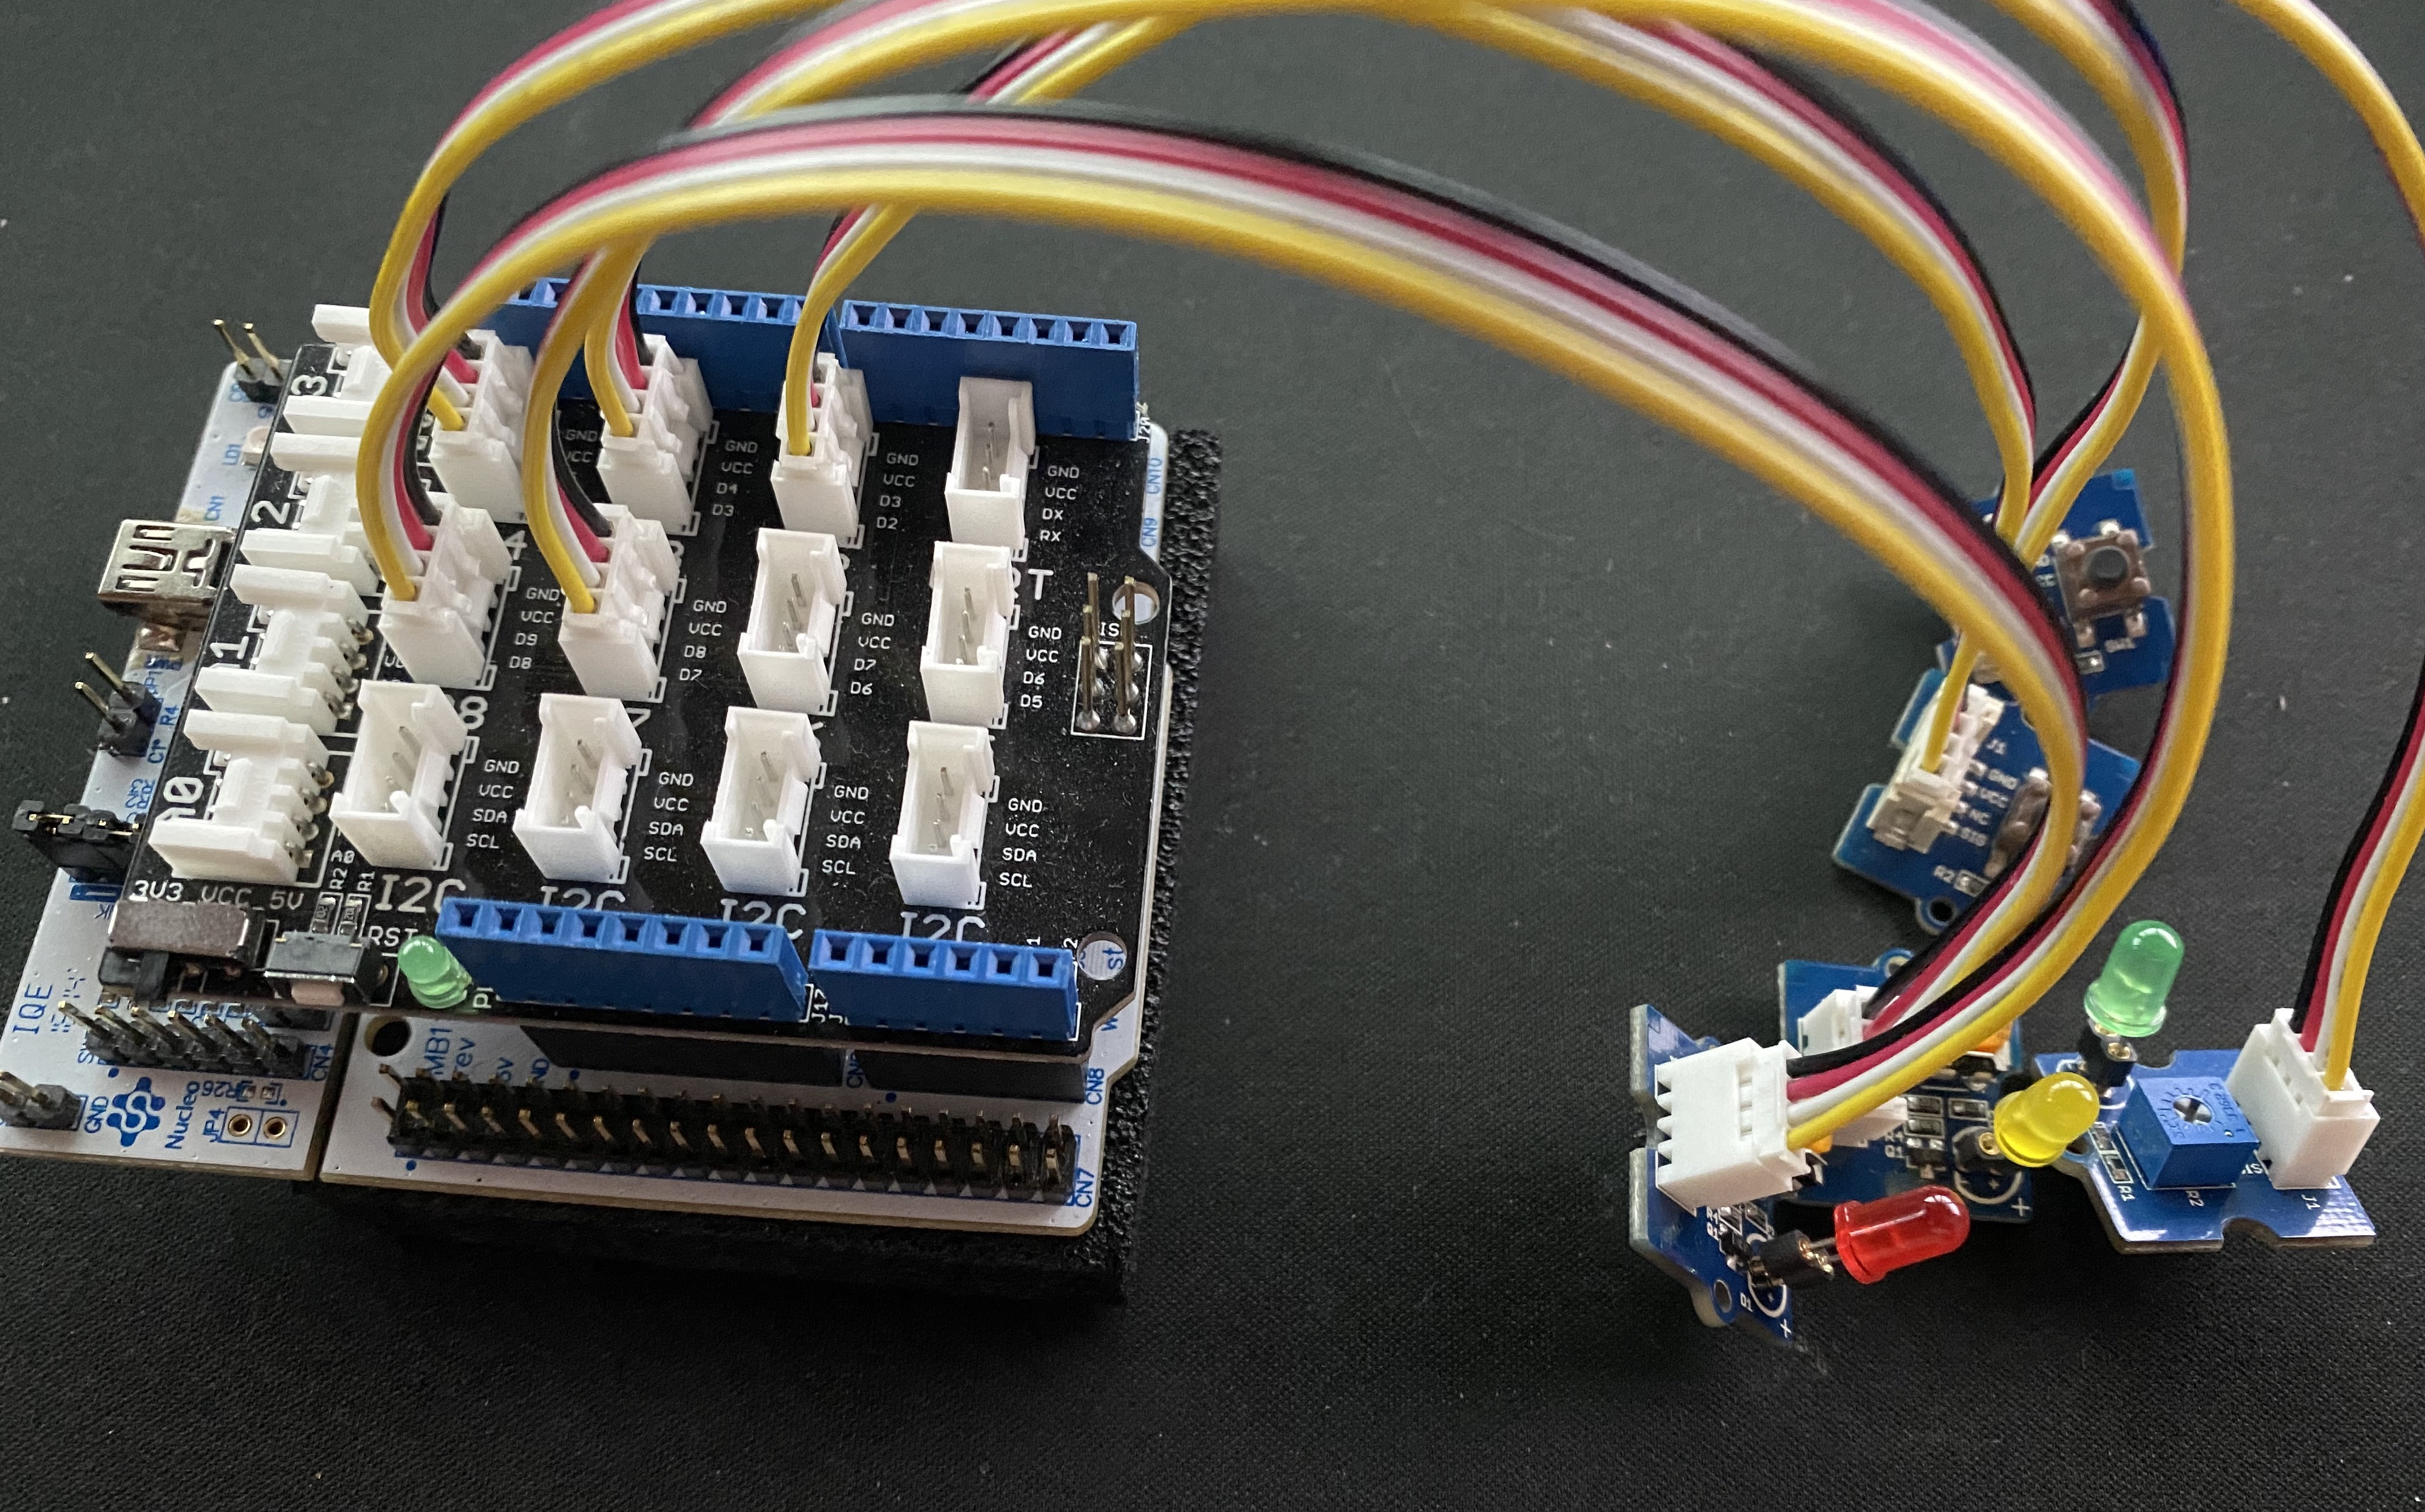
\includegraphics[width=0.38\textwidth]{images/02.png}
	\caption{Hardwareaufbau der Ampelsteuerung  \protect \\ Quelle: Eigene Darstellung }
	\label{fig:grafik2}
\end{figure}


\section{Pinbelegung}
Da der Arbeitsaufwand dieses Projektes auf vier Studierende aufgeteilt wird, muss abgestimmt werden, welcher Pin jeweils den LEDs und den Buttons zugeordnet werden soll. Deshalb wird gleich zu Beginn des Projektes eine Vereinbarung der Pinbelegungen getroffen. Diese ist in \autoref{tab:Pinbelegung} zu sehen.\\

\begin{table}[H]
\centering
\begin{tabular}{c|c|l}
	Hardware - Shield & Software (Port Pin) & Bauteil \\
	\hline
	\rule{0pt}{20pt}D7 & A8 & LED Rot \\
	D8 & A9 & LED Gelb \\
	D2 & A10 & LED Grün \\
	D3 & B3 & Taster 1 \\
	D4 & B5 & Taster 2 \\
	
\end{tabular}
\caption{Pinbelegung (Hardware/Software)}
\label{tab:Pinbelegung}
\end{table}


	\newpage
	\input{content//03.tex}
	\newpage
	\chapter{Systemarchitektur}
\section{Klassendiagramm des Projekts}

In diesem Abschnitt wird das Klassendiagramm der Ampelschaltung (siehe Abbildung \ref{fig:grafik8}) erläutert. Es wird darauf eingegangen, wie die einzelnen Klassen in Beziehung zueinanderstehen und wie diese gruppiert werden können.\\
\\
Das Klassendiagramm lässt sich in vier Bereiche unterteilen:\\

\begin{itemize}
	\item Auswahl Betriebsmodus (blau)
	\item Steuerung Farben (grün)
	\item Output (rot)
	\item Input (schwarz)\\
\end{itemize}

Der Bereich \glqq Auswahl Betriebsmodus\grqq{} bildet die Logik der beiden Betriebsmodi ab, in denen sich die Ampel befinden kann. Zum einen der aktive Modus, in welchem die Ampel die Farben durchschaltet und zum anderen den Modus, in welchem die Ampel orange blinkt. Der Bereich \glqq Steuerung Farben\grqq{} übernimmt die Aufgabe die Zustände im Hinblick auf die Farben der Ampel bereitzustellen. Die Ampel kann Rot ausgeben, Rot-Orange, Orange, Grün oder ausgeschaltet sein. Der Output übernimmt die Funktion, die einzelnen Farben zu setzen und dies entweder software- oder hardwaremäßig. Der Input übernimmt die Aufgabe die Benutzereingabe bereitzustellen, die ebenso entweder software- oder hardwaremäßig eingegeben werden kann. Die Klasse GPIO, die nicht in einen der Bereiche zugeordnet wird, bildet die Schnittstelle für den Hardwarezugriff ab.\\
\\
Hierarchisch ganz oben ist die Kontextklasse \glqq Traffic Light\grqq{} zu sehen. Ein Objekt dieser Klasse wird in der\: \texttt{main()} erstellt und beinhaltet die Logik der gesamten Ampelschaltung. Wird die\: \texttt{Handle()} Funktion dieses Objekts aufgerufen, läuft die Ampelschaltung wie gefordert ab. Die Aufgabe Benutzereingaben einzulesen wird an das Interface \glqq InputFormat\grqq{} delegiert. Je nachdem, ob eine Hardware angeschlossen ist, liefern die Klassen \glqq SoftwareInput\grqq{} und \glqq HardwareInput\grqq{} den jeweiligen Tasterwert, bzw. die Tastatureingabe. Die Klasse \glqq UserButtons\grqq{} frägt beide Pins (für die beiden Taster) ab und stellt der Klasse \glqq HardwareInput\grqq{} nur einen Wert zur Verfügung, der die beiden Tasterzustände abbildet. Damit die Klasse \glqq UserButtons\grqq{} auf die Registerinhalte des Mikrocomputers zugreifen kann, steht sie in Beziehung mit der Klasse \glqq GPIO\grqq{}. Ein Objekt der \glqq Traffic Light\grqq{} Klasse kann den Zustand in Betrieb oder außer Betrieb annehmen. Über das Interface \glqq state\grqq{} werden die Zustandsklassen \glqq flashing\grqq{} und \glqq active\grqq{} hierfür bereitgestellt. Diese beiden Klassen greifen über das Interface \glqq LightControl\grqq{} auf die Farbenklassen \glqq Off\grqq{}, \glqq Red\grqq{}, \glqq RedAmber\grqq{}, \glqq Amber\grqq{} und \glqq Green\grqq{} zu. Diese Unterklassen sind dafür verantwortlich, dass die Ampel den Farbzustand annimmt. Des Weiteren bieten diese Klassen die Funktion an, Objekte für den nächsten Farbzustand zurückzuliefern. Noch eine Hierarchieebene weiter darunter greifen die Farbklassen über das Interface \glqq OutputFormat\grqq{} auf die \glqq SoftwareOutput\grqq{} bzw. auf die Klasse \glqq HardwareOutput\grqq{} zu. Diese realisieren die Ausgabe der Ampelschaltung. Im Fall, dass Hardware angeschlossen ist, greift die \glqq HardwareOutput\grqq{} Klasse über die \glqq UserLEDs\grqq{} Klasse auf die \glqq GPIO\grqq{} Klasse zu. Damit werden die entsprechenden Bits in den Registern des Mikrocontrollers gesetzt, damit die entsprechenden Pins der LEDs auf HIGH geschaltet werden können.

\begin{figure}[H] 
	\centering
	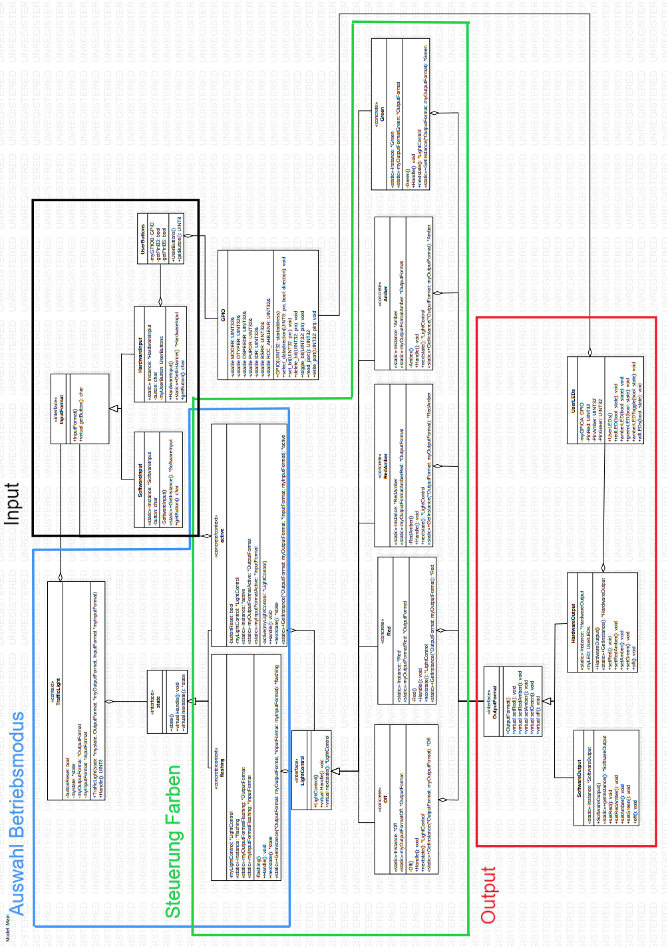
\includegraphics[width=0.95\textwidth]{images/08.png}
	\caption{Klassendiagramm der Ampelsteuerung \protect \\ Quelle: Eigene Darstellung }
	\label{fig:grafik8}
\end{figure}

\section{Zustandsautomat}

\begin{figure}[H] 
	\centering
	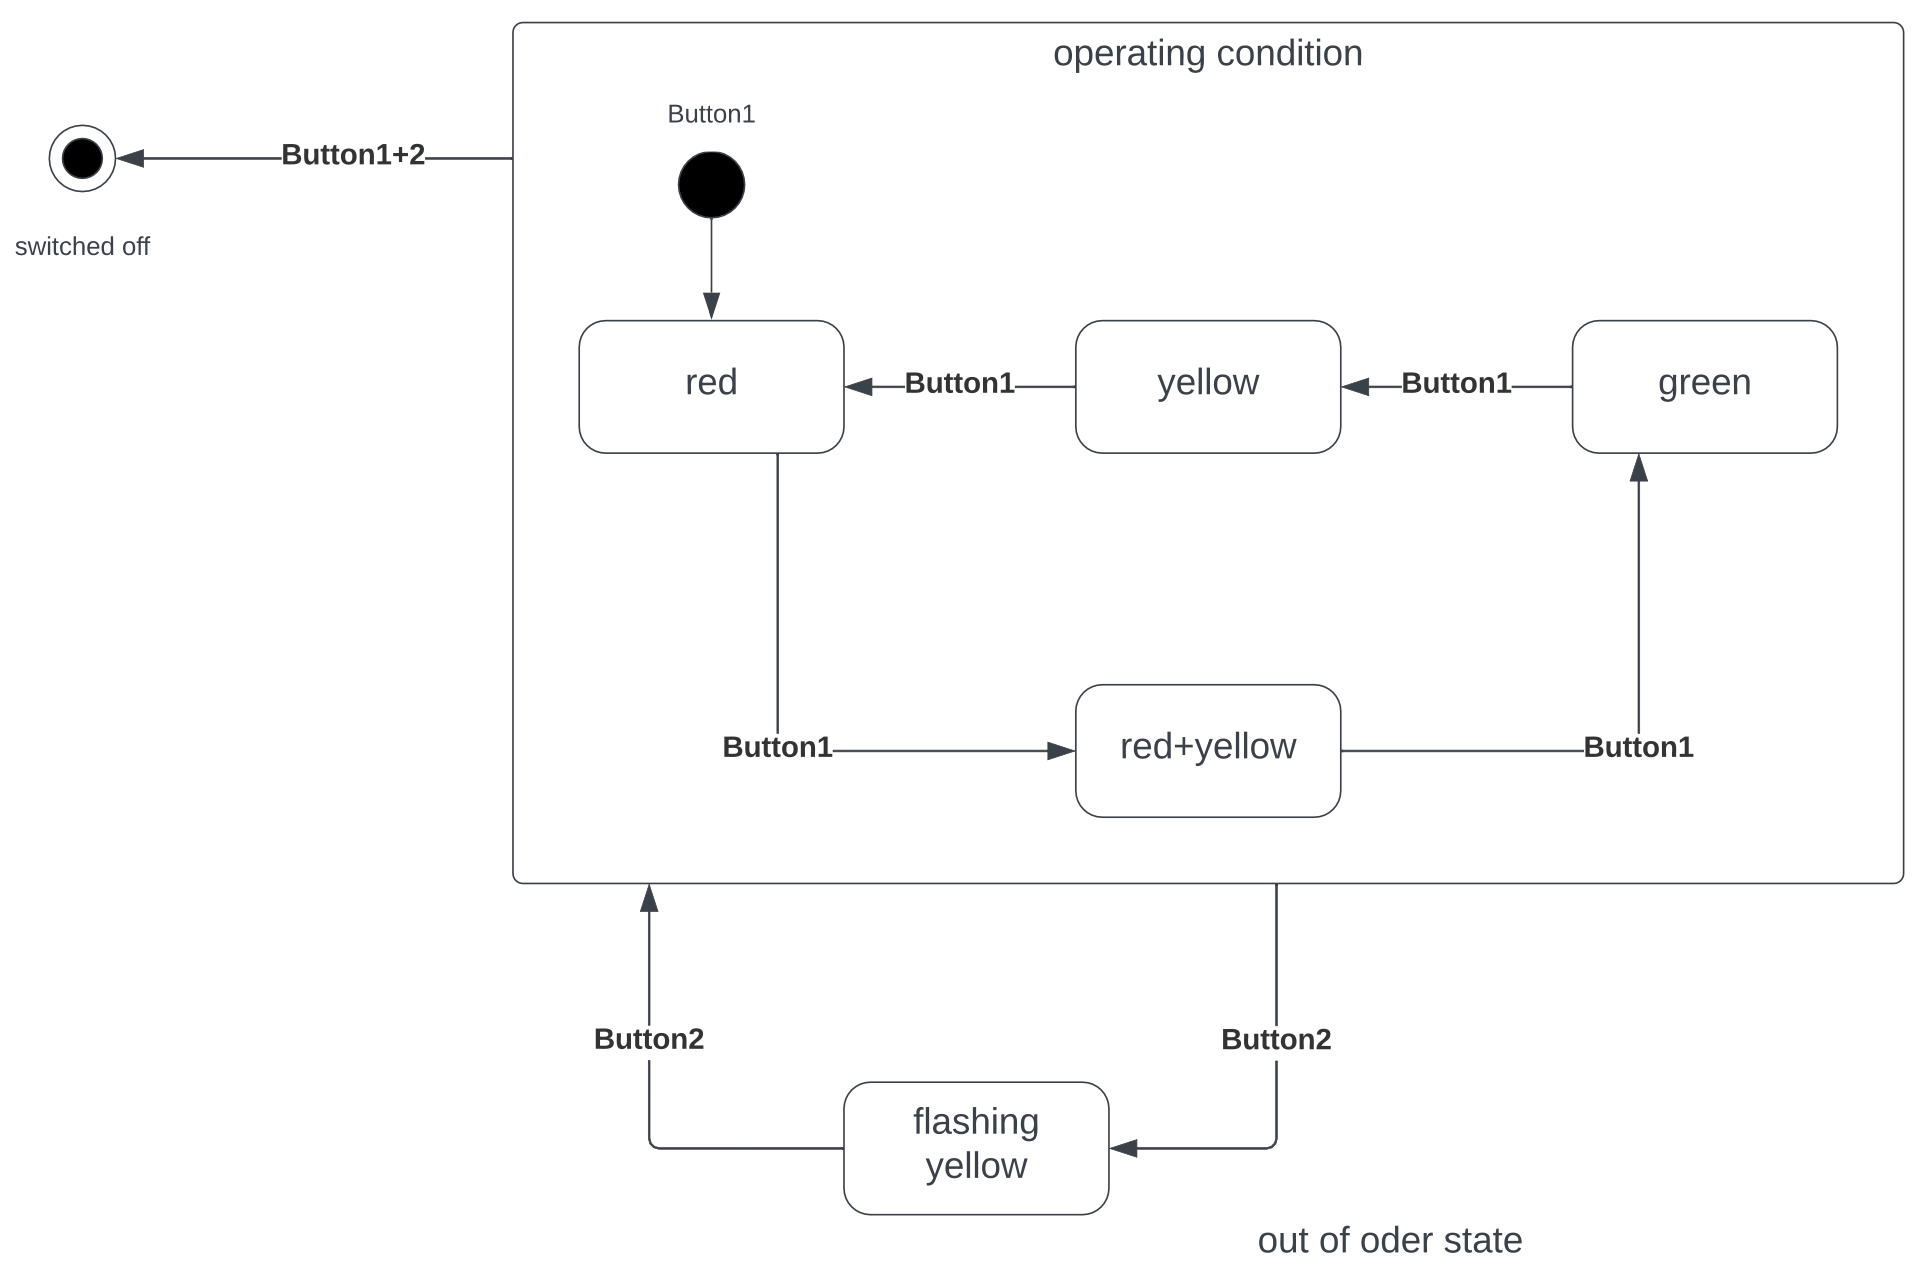
\includegraphics[width=1.0\textwidth]{images/03.png}
	\caption{Zustandsautomat der Ampelsteuerung \protect \\ Quelle: Eigene Darstellung }
	\label{fig:grafik3}
\end{figure}


Ein Zustandsdiagramm ist eines der 14 Diagrammarten der Sprache UML für Software und andere Systeme. Es ermöglicht dem Entwickler sich einen Gesamtüberblick über die Zustände und Operationen, welche in einem Projekt/Programm erfolgen sollen, zu verschaffen. \\
Die zu implementierende Ampelsteuerung soll zwei Zustände \glqq In Betrieb\grqq{} und \glqq Außer Betrieb\grqq{} annehmen können. Im Betrieb soll die Ampelsteuerung die Ampelphasen Rot, Rot-Gelb, Grün und Gelb durchlaufen (siehe \autoref{fig:grafik3}). Die Ampelphasen sollen per Taster \glqq T1\grqq{} oder Tastatureingabe \glqq F\grqq{} gesteuert werden. Zwischen jeder Ampelphase kann die Ampelsteuerung mit dem Taster \glqq T2\grqq{} oder Tastatureingabe \glqq B\grqq{} in den \glqq Außer Betrieb\grqq{} Zustand gesetzt werden. Innerhalb dieses Zustandes, soll die gelbe LED blinken (siehe \autoref{fig:grafik3}). Immer wenn die Ampelsteuerung neugestartet oder in den Betriebsmodus \glqq In Betrieb\grqq{} wechselt, soll sie in der roten Ampelphase starten.

	\newpage
	\chapter{State Pattern}
Nachfolgend wird das eingesetzte Design Pattern State erläutert.
\section{Context, Interface und Concrete Klassen}
In der vorliegenden Ampelschaltung werden zwei State Patterns verwendet. Zudem wird beim Input und Output sich eines Interfaces bedient, welches Polymorphie zulässt. Das heißt, je nachdem ob Hardware angeschlossen ist, werden die Hardware oder Software Klassen verwendet. Näheres dazu wird in dem Kapitel \glqq Wechsel zwischen Hardware- und Softwarebetrieb\grqq{} beschrieben. Das hierarchisch höhere State Pattern besteht aus der Kontextklasse \glqq TrafficLight\grqq{}, dem Interface \glqq state\grqq{} und den Concrete Klassen \glqq flashing\grqq{} und \glqq active\grqq{}. Je nach Benutzereingabe verweist der Zeiger vom Typ \glqq state\grqq{} auf eine Instanz der Klasse \glqq flashing\grqq{} oder \glqq active\grqq{}. Wird die Handle Funktion des Interfaces aufgerufen, ist die Ampel entweder im konkreten Zustand \glqq in Betrieb\grqq{} oder \glqq außer Betrieb\grqq{}. Fordert der Benutzer ein Wechsel des Betriebsmodus, so ist der nächste Zustand der jeweils andere Betriebsmodus. Das zweite State Pattern wechselt zwischen den Farbzuständen. Dieses State Pattern besteht entweder aus der Kontextklasse \glqq flashing\grqq{} oder \glqq active\grqq{}, dem Interface \glqq LightControl\grqq{} und den Concrete Klassen (\glqq Off\grqq{}, \glqq Red\grqq{}, \glqq RedAmber\grqq{}, \glqq Amber\grqq{},  \glqq Green\grqq{}). Die Klasse  \glqq active\grqq{} ruft die Funktionen \glqq nextstate\grqq{} des Interfaces auf, damit die Ampelfarben durchgeschaltet werden. Im außer Betrieb Zustand wechselt der Farbzustand der Ampel zwischen Off und Amber.

\section{Singleton}
Das Singleton Design Pattern hilft in der objektorientierten Programmierung dem Entwickler mit vielfachen Vorlagen das Lösen von Programmieraufgaben. Es ist sehr leistungsfähig und gehört zu der Kategorie der Erzeugungsmuster unter den Design Pattern. Der Ausdruck Singleton wird oftmals als \glqq Einzelstück\grqq{} betitelt. Dieses Synonym bildet sehr gut die Funktion einens Singeltons ab, da die Aufgabe darin besteht nicht mehr als ein Objekt einer Klasse zu erstellen. Wurde mit der Klasse über das Singleton Pattern nur eine Instanz der Klasse erzeugt, sorgt es auch dafür, dass es ledlich bei dieser einen Instanz der Klasse bleibt. Oftmals dient eine Funktion, wie \texttt{GetInstance} dafür, dass nur eine Instance der Klasse erstellt wird.\\
\\
Im Bezug auf die Ampelsteuerung wurde das Singleton Pattern in sieben unterschiedlichen Klassen verwendet. Diese lauten wie folgt:

\begin{itemize}
	\item active.h
	\item flashing.h
	\item Red.h
	\item Amber.h
	\item RedAmber.h
	\item Green.h
	\item Off.h
\end{itemize}

Da der Aufbau in jeder Klasse identisch ist, folgt die Erläuterung im Code nun am Beispiel der Klasse \texttt{Red.h}.\\

\begin{figure}[H] 
	\centering
	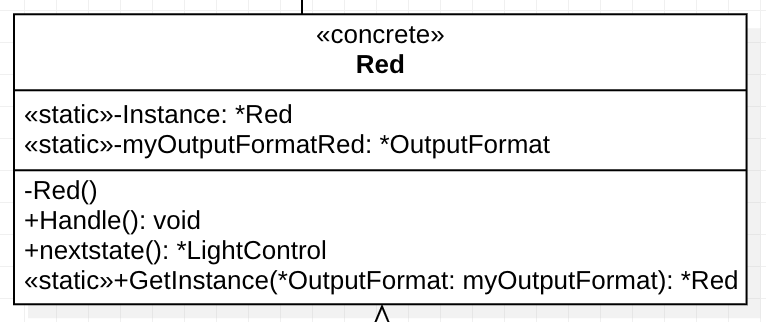
\includegraphics[width=0.7\textwidth]{images/07.png}
	\caption{Singleton Patten am Beispiel der Red.h Klasse \protect \\ Quelle: Eigene Darstellung }
	\label{fig:grafik7}
\end{figure}

In der \autoref{fig:grafik7} sind die Funktionen und Instanzen der Red.h Klasse zu sehen, welche mit Hilfe des Singleton Pattern implementiert wurde. Das Schlüsselwort \texttt{static} bedeutet einmal, dass die als \texttt{static} deklarierte Variable oder Funktion ihren Wert innerhalb zwischen Aufrufen behält und andermal, dass eine globale statische Variable oder Funktion nur in der Datei \glqq gesehen\grqq{} wird, in der sie deklariert wurde. Um das Singleton Pattern nutzen zu können, wird die statische Instanz und die Funktion \texttt{GetInstance} benötigt. Die Funktion \texttt{GetInstance} hat die Aufgabe, bei jedem Aufruf eine Instance zu erzeugen (siehe \autoref{codeauszug:red.h1}). \\

\begin{lstlisting}[style=myC,caption={Red.cpp - Singleton in der Klasse Red},label={codeauszug:red.h1},captionpos=b]
	...
	Red *Red::Instance = NULL;
	
	Red *Red::GetInstance(OutputFormat *myOutputFormat)
	{
		myOutputFormatRed = myOutputFormat; 
		if (Instance == NULL)
		{
			Instance = new Red();
		}
		return Instance;
	}
	...
\end{lstlisting}

Wie in Zeile 2 zu erkennen ist, wird die Instanz der Klasse immer auf \texttt{NULL} deklariert. In Zeile 4 der cpp-Datei wird ist die Implementierung der Funktion \texttt{GetInstance} zu sehen. Innerhalb dieser Funktion wird der übergebene Parameter \texttt{myOutputFormat} der Klasse Red zugeweisen. Folgend findet eine \texttt{if} Überprüfung statt, ob es schon eine Instance der Klasse Red.h gibt. Wenn nicht, wird in Zeile 9 eine neue Instanz der Klasse Red.h erzeugt. Anschließend besitzt die Funktion \texttt{GetInstance} als \texttt{return}-Wert die erzeugte Instanz. Wichtig ist es, dass die statische Instanz als \texttt{private} und die Funktion \texttt{GetInstance} als \texttt{public}.

\chapter{Hardwarezugriff - GPIO}
Der Hardwarezugriff erfolgt über drei Klassen. Die untergeordnete Klasse \texttt{GPIO} greift dabei direkt auf die Register des Mikrocontrollers zu und steuert somit sämtliche Hardwarezugriffe. Die zwei übergeordneten Klassen \texttt{UserLEDs} und \texttt{UserButtons} greifen dann auf die Klasse \texttt{GPIO} zu und steuern diese. Übergeordnet heißt hier jedoch nicht, dass es sich um Oberklassen einer Vererbung handelt. Die hier herrschende Beziehung ist eine Aggregation. Außer zu diesen beiden Klassen hat die \texttt{GPIO}-Klasse keine weiteren Verbindungen. Eine Hardwareansteuerung kann somit nur durch die beiden genannten übergeordneten Klassen durchgeführt werden.\\
\\
Nun wird etwas genauer auf die die \texttt{GPIO}-Klasse eingegangen. Sie ist wie folgt aufgebaut:

\begin{figure}[H] 
	\centering
	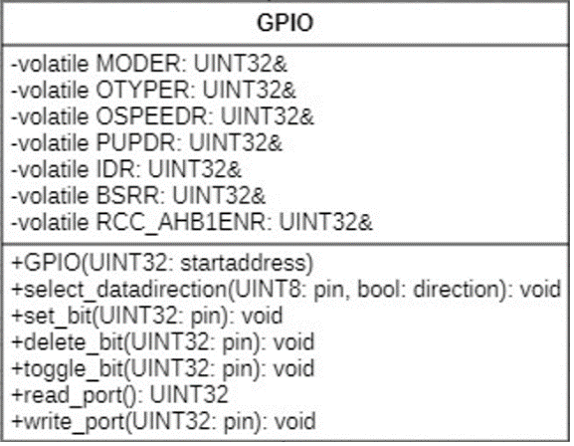
\includegraphics[width=0.5\textwidth]{images/04.png}
	\caption{GPIO Klasse \protect \\ Quelle: Eigene Darstellung}
	\label{fig:grafik4}
\end{figure}

Alle Attribute dieser Klasse sind als \glqq private\grqq{} gekennzeichnet. Das liegt daran, dass es sich bei den Attributen um Zeiger handelt, mit welchen man auf die GPIO-Register des Mikrocontrollers zugreifen kann. Hier wird das Prinzip des Information Hidings angewendet, um zu verhindern, dass die Register von außen manipuliert werden könnten. Weiterhin wird den Attributen das Schlüsselwort volatile vorangestellt. Dieses gibt dem Compiler die Information, dass sich der Inhalt auf den die Zeiger zeigen, ändern kann, auch wenn das Programm nicht schreibend darauf zugreift.\\
\\
Der Konstruktor der Klasse konfiguriert einen GPIO-Port. Ihm muss lediglich die Startadresse des gewünschten Ports übergeben werden. Diese Startadresse kann dem Datenblatt auf Seite 53 entnommen werden. Auf Basis der Startadresse adressiert dieser dann die benötigten Register. Weiterhin wird dort das Clock Signal des ausgewählten Ports aktiviert.
Über die Methode \texttt{select\_datadirection()} kann dann für jeden Pin des Ports einzeln ausgewählt werden ob, dieser als Input oder als Output fungieren soll. Dazu muss der Methode nur die Pinnummer und die Art des GPIOs übergeben werden.
Mit \texttt{set\_bit()} kann ein ausgewählter Output gesetzt werden. Dazu muss lediglich die Pinnummer bekannt sein. \texttt{delete\_bit()} macht genau das Gegenteil. Dort wird ein Output zurückgesetzt. \texttt{toggle\_bit()} vereint beide Methoden. Dort wird der Status des Outputs abgefragt und danach umgekehrt.
Mit \texttt{read\_port()} werden die Zustände jedes einzelnen Pins des gesamten Ports gelesen und als 32-Bit Wert zurückgeben. Bei der Ausführung von \texttt{write\_port()} hingegen, wird der gesamte Port beschrieben. Wirksam ist der Schreibzugriff jedoch nur auf definierte Outputs.\\
\\
Nun wird auf die Klasse \glqq UserLEDs\grqq{} betrachtet. Das dazugehörige Klassendiagramm kann folgender Abbildung entnommen werden: \\

\begin{figure}[H] 
	\centering
	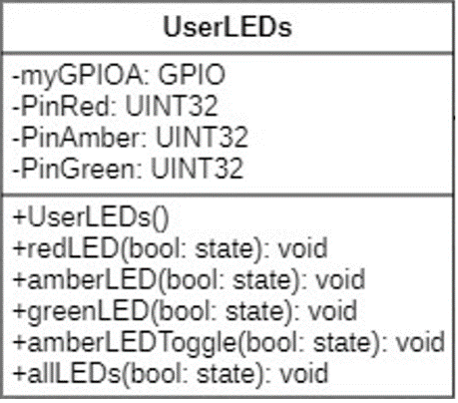
\includegraphics[width=0.35\textwidth]{images/05.png}
	\caption{UserLEDs Klasse \protect \\ Quelle: Eigene Darstellung}
	\label{fig:grafik5}
\end{figure}

Auch hier sind alle Attribute als private definiert, um das Information Hiding zu waren. Das erste Attribut ist eine Instanz der \texttt{GPIO}-Klasse. Es dient als Schnittstelle zur Ansteuerung der Pins, an welchen die LEDs angeschlossen sind. In den restlichen drei Attributen werden die jeweiligen Pinnummern der LEDs hinterlegt. Dies erfolgt im Konstruktor über eine Initialisierungsliste. Danach wird dort noch, über die \texttt{select\_datadirection()}-Methode der \texttt{GPIO}-Klasse festgelegt, dass es sich bei den vorliegenden Pins um Outputs handelt. Mit den restlichen Methoden werden dann die LEDs angesteuert. Ihnen muss lediglich der gewünschte Zustand übergeben werden.\\
\\
Zuletzt wird die Klasse \texttt{UserButtons} betrachtet. Auch hier wird ein UML Klassendiagramm zur Erläuterung herbeigezogen:\\

\begin{figure}[H] 
	\centering
	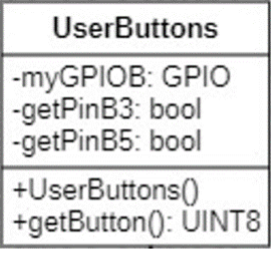
\includegraphics[width=0.2\textwidth]{images/06.png}
	\caption{UserButtons Klasse \protect \\ Quelle: Eigene Darstellung }
	\label{fig:grafi6}
\end{figure}

Dort wird auch wieder eine private Instanz der Klasse \texttt{GPIO} erstellt. Damit können die Buttons abgefragt werden. Weiterhin existieren zwei private Methoden, welche den Status des jeweiligen Buttons zurückgeben. Sie werden in der Methode \texttt{getButton()} aufgerufen. Dort erfolgt eine Entprellung. Dazu wird der Wert zunächst ein erstes Mal abgefragt. Danach wird 3000 Schleifendurchgänge gewartet und der Status erneut abgefragt. Liefern beide Abfragen das gleiche Ergebnis, so wird der Wert übernommen. Andernfalls wird die Entprellung erneut durchgeführt. Wie im Klassendiagramm zu sehen hat die Methode einen Rückgabewert vom Datentyp \texttt{UINT8}, dies entspricht einem 8 Bit Charakter. Je nachdem, welcher Button nun gedrückt wird, wird ein bestimmter Rückgabewert zurückgegeben. Eine Auflistung aller möglichen Rückgabewerte kann folgender \autoref{tab:Rueckgabe} entnommen werden:\\

\begin{table}[H]
	\centering
	\begin{tabular}[H]{c|c}
	Welche Buttons gedrückt? & Rückgabewert \\
	\hline
	Keiner & O \\
	Nur Button an B3 (D3) & B \\
	Nur Button an B5 (D4) & F \\
	Beide Buttons &  X \\
	\end{tabular}
	\caption{Rückgabewerte Buttons}
	\label{tab:Rueckgabe}
\end{table}

\chapter{Wechsel zwischen Hardware- und Softwarebetrieb}
Nachstehend wird die Umsetzung der Wechsels zwischen Hardware- und Softwarebetrieb erläutert.
\section{Definition}
Wie bereits erwähnt, soll es dem Anwender möglich sein, die Ampelsteuerung sowohl mit Hardware, als auch komplett ohne Hardware nutzen zu können. Um die beiden Fälle näher zu erläutern, wird der Hardware- und Softwarebetrieb im Folgenden konkret spezifiziert.

\begin{itemize}
	\item \textbf{Hardwarebetrieb:} Der Programmcode der Ampelsteuerung wird auf das Nucleo Board geflasht und auf diesem ausgeführt. Die Nutzereingabe erfolgt über zwei an das Board angeschlossenen Taster. Die Ausgabe der Ampelfarben erfolgt über die drei angeschlossenen LEDs.
	\item \textbf{Softwarebetrieb:} Das Programm der Ampelsteuerung wird auf dem PC ausgeführt. Die Nutzereingabe erfolgt über die Tastatur. Die Tasten \glqq F\grqq\:und \glqq B\grqq\:repräsentieren die beiden Hardwaretaster. Die Taste \glqq X\grqq\:steht für das Betätigen beider Taster gleichzeitig. Das Einlesen der Tastatureingaben erfolgt über den Eingabestream \texttt{cin}, die Ausgabe der Ampelfarben über den Ausgabestream \texttt{cout} in der Kommandozeile.
\end{itemize}

\section{Umsetzung}
Ob die Ampelsteuerung im Hardware- oder Softwarebetrieb arbeitet, wird über Pointer bestimmt, welche in der \:\texttt{main.cpp}\: des Programmes angelegt und bis zur relevanten Stelle im Programmcode durch alle Klassen übergeben werden. Ob die Pointer für den Hardware- oder Softwarebetrieb initialisiert werden, wird wiederum über eine Präprozessoranweisung festgelegt, welche der Nutzer setzen oder auskommentieren kann. Dies ist in \autoref{codeauszug:HWSW} dargestellt. \\

\begin{lstlisting}[style=myC,caption={main.cpp - Hardwarebetrieb oder Softwarebetrieb},label={codeauszug:HWSW},captionpos=b]
...
#define _HARDWAREPRESENT
int main(){
	#ifdef _HARDWAREPRESENT
		OutputFormat *myOutputFormat = HardwareOutput::GetInstance();
		InputFormat *myInputFormat = HardwareInput::GetInstance();
	#else
		OutputFormat *myOutputFormat = SoftwareOutput::GetInstance();
		InputFormat *myInputFormat = SoftwareInput::GetInstance();
	#endif
...
\end{lstlisting}

Im weiteren Programmcode wurde die Umschaltung zwischen Hardware- und Softwarebetrieb nochmals aufgeteilt. Zum einen wird beim Ausgabeformat der Ampelfarben zwischen Hardware- und Softwareausgabe, zum anderen beim Eingabeformat der Nutzereingabe zwischen Hardware- und Softwareeingabe unterschieden.
\subsection{Ausgabeformat}
\autoref{fig:output} zeigt den Ausschnitt aus dem Klassendiagramm, welcher für die Umschaltung zwischen Hardware- und Softwareausgabe zuständig ist.
Die Klasse \glqq OutputFormat\grqq\:ist eine Interface Klasse und beinhaltet ausschließlich virtuelle Methoden. Die Unterklassen \glqq SoftwareOutput\grqq\:und \glqq HardwareOutput\grqq\:erben von der Oberklasse \glqq OutputFormat\grqq\:und verwenden deren Interface. 
Die Concrete Klassen des übergelagerten State Patterns, welche die unterschiedlichen Ampelfarben repräsentieren, besitzen den erläuterten übergebenen Zeiger, welcher in der \:\texttt{main.cpp}\: initialisiert wurde und auf eine Instanz der Klasse \glqq HardwareOutput\grqq\:oder \glqq SoftwareOutput\grqq\:zeigt. Je nachdem werden die Methoden von \glqq HardwareOutput\grqq\:oder \glqq SoftwareOutput\grqq\: aufgerufen, um die Ampelfarben hardware- oder softwareseitig anzuzeigen.

 Beim Hardwarebetrieb ruft die Klasse \glqq HardwareOutput\grqq\:schließlich die Methoden der Klasse \glqq UserLEDs\grqq\:auf und steuert so die LEDs an. Befindet sich die Ampelsteuerung im Softwarebetrieb, so sorgen die Methoden in der Klasse \glqq SoftwareOutput\grqq\:für die entsprechenden Ausgabestreams in der Kommandozeile.\\

\begin{figure}[H] 
	\centering
	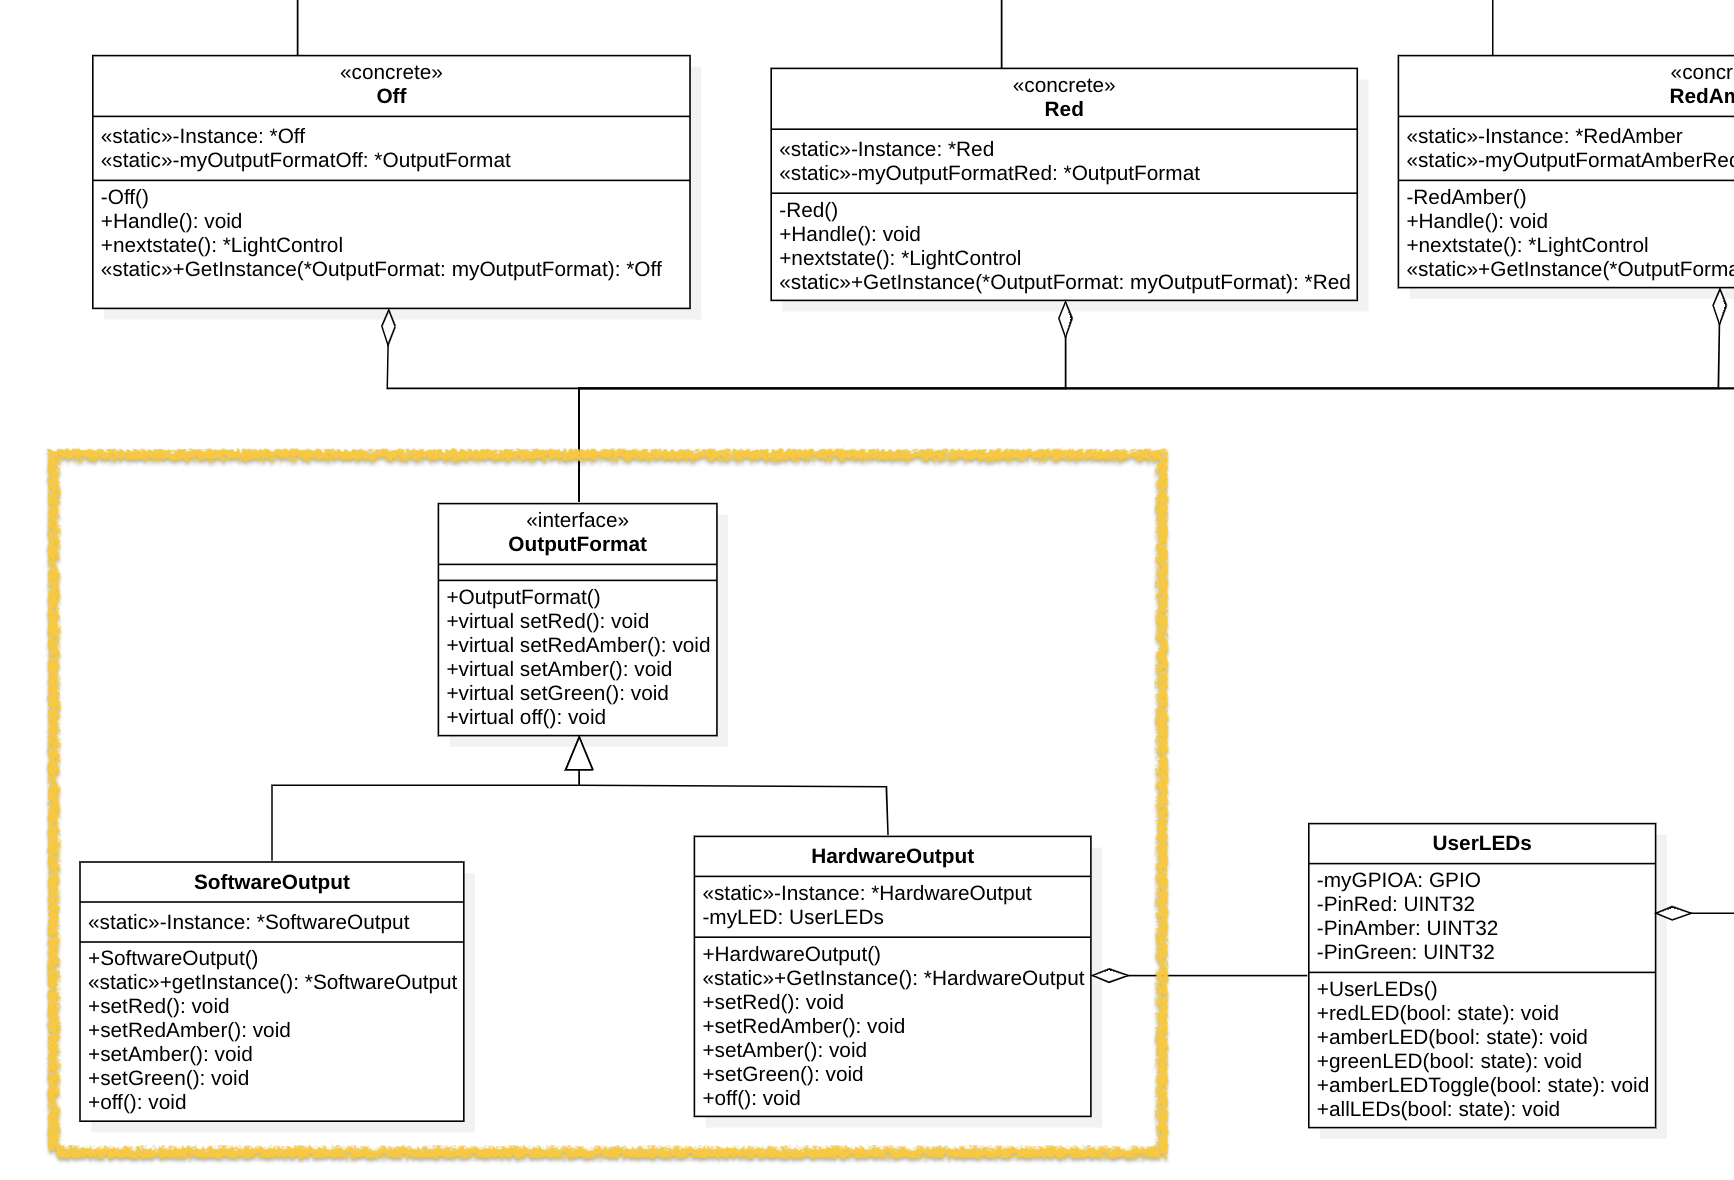
\includegraphics[width=1.0\textwidth]{images/Outputformat}
	\caption{Auszug aus dem Klassendiagramm - Ausgabeformat \protect \\ Quelle: Eigene Darstellung 
	 }
	\label{fig:output}
\end{figure}

\subsection{Eingabeformat}
\autoref{fig:input} zeigt einen Auszug aus dem Klassendiagramm, welcher für den Wechsel zwischen Hardware- und Softwareeingabe zuständig ist. 
Auch hier sind eine Interface Klasse \glqq InputFormat\grqq\: und zwei erbende Unterklassen \glqq HardwareInput\grqq\:und \glqq SoftwareInput\grqq, welche das Interface verwenden, vorzufinden. Der Wechsel zwischen Hardware- und Softwareeingabe funktioniert dabei identisch zur Logik der Hardware- und Softwareausgabe, weshalb darauf an dieser Stelle nicht weiter eingegangen wird.
\\
\begin{figure}[H] 
	\centering
	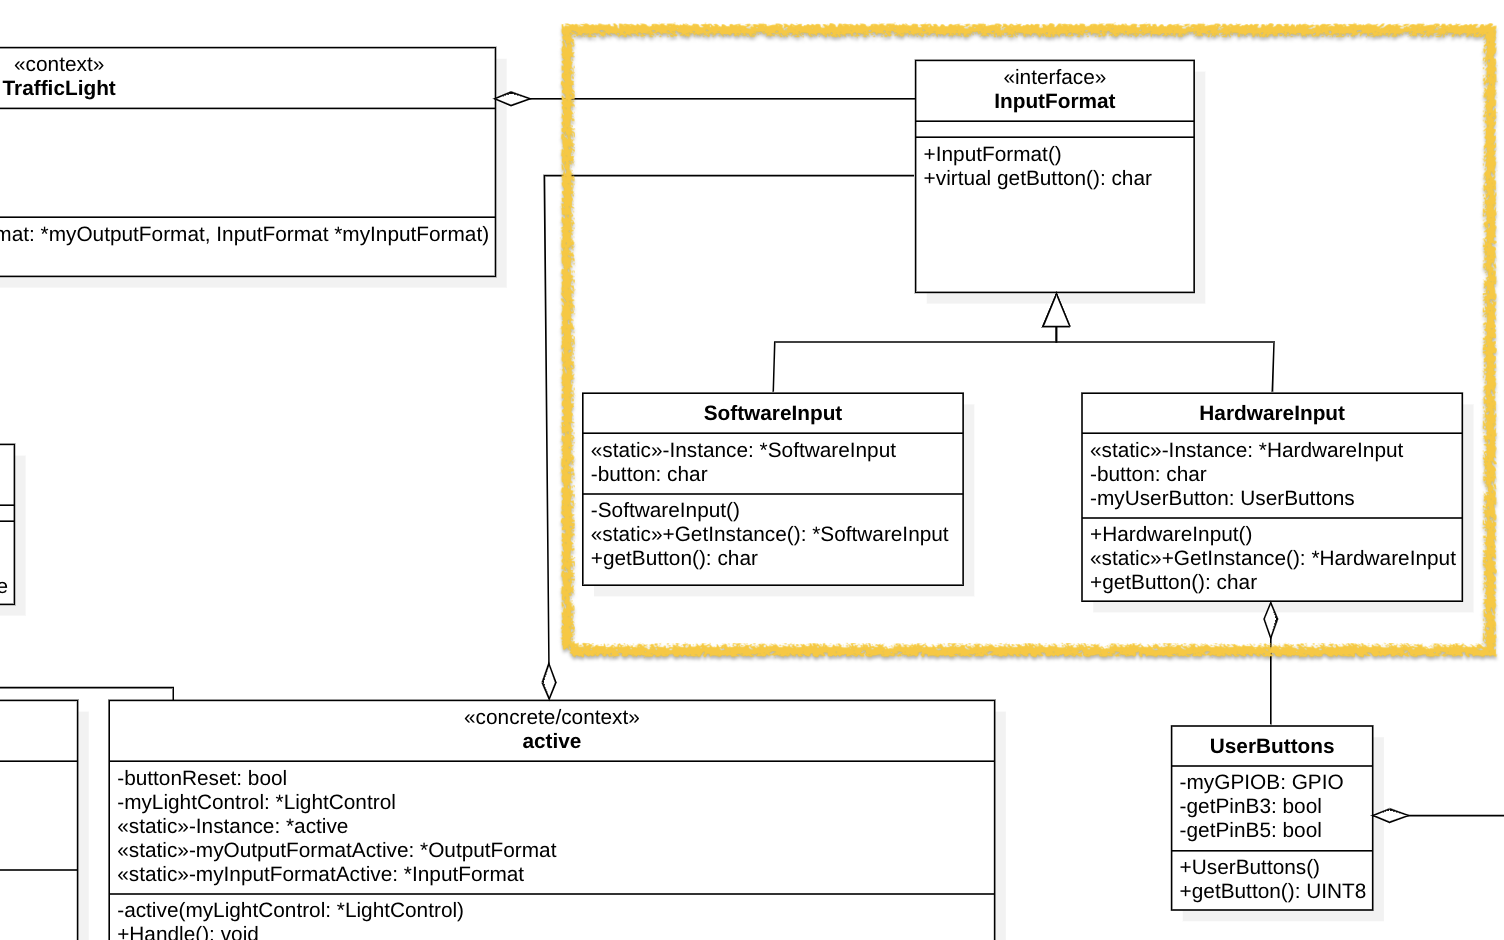
\includegraphics[width=1.0\textwidth]{images/Inputformat}
	\caption{Auszug aus dem Klassendiagramm - Eingabeformat \protect \\ Quelle: Eigene Darstellung }
	\label{fig:input}
\end{figure}

\chapter{Bedienungsanleitung}
Im Folgenden wird erläutert, wie die Ampel in der IAR Embedded Workbench zu betreiben ist. Vorausgesetzt wird, dass die Hardware per USB an den PC angeschlossen ist und die LEDs, bzw. die Taster in der richtigen Pinbelegung mit dem Board verbunden sind. Im Default Zustand geht die Ampelschaltung davon aus, dass Hardware angeschlossen ist. Wird nun das Projekt ausgeführt, so kann die Ampel über die Hardware Taster bedient werden und die Hardware LEDs leuchten entsprechend auf. Steht dem Benutzer keine Hardware zur Verfügung, so muss die Zeile „define \_HARDWAREPRESENT“ in der Main Datei auskommentiert werden. Die Ampel kann jetzt mit der Tastatur bedient werden und die Ausgabe erfolgt über das Terminal der IAR Embedded Workbench. Die Eingabe erfolgt ebenso über das Terminal des Programms. Hier kann auch die Beispiel Textdatei „Input.txt“ als Eingabe geladen werden. Die Textdatei befindet sich in den Quellcode Dateien. Die Ampel durchläuft im Beispiel zunächst alle Farbzustände im „in Betrieb“ Modus und wechselt, dann in den „außer Betrieb“ Modus. Wichtig bei der Eingabe ist, dass die Buchstaben „O“, „F“, „B“ und „X“, so eingegeben werden, als würden die entsprechenden Taster gedrückt werden. Das heißt nach jedem Buchstaben muss wieder „O“ folgen, da der Taster losgelassen wird. Auch müssen die Buchstaben öfters eingegeben werden, damit das Programm weiterläuft.


\chapter{Fazit}
Abschließend lässt sich sagen, dass die Aufgabenstellung mit dem vorliegenden Projekt erfüllt ist. Die implementierte Ampelsteuerung verfügt über alle vorgeschriebenen Funktionen. Beide definierte Betriebszustände, der „in Betrieb“ Modus und der „nicht in Betrieb“ Modus sind wie gefordert, umgesetzt. Des Weiteren kann die Ampel softwaremäßig und hardwaremäßig ausgeführt werden. Zudem sind die geforderten Methoden, Werkzeuge und Prinzipien der UML und der C++ Programmierung, die in der Vorlesung behandelt worden sind, in das Projekt eingeflossen und sinnvoll umgesetzt worden. Meiner Meinung nach hat das Projekt sehr viel Spaß gemacht und hat einen persönlich in der objektorientierten Programmierung weitergebracht. Durch das Projekt konnte eine zustandsorientierte Aufgabe objektorientiert mit der Sprache C++ umgesetzt werden.


	\newpage


	
	
	
	\pagenumbering{Roman}
	\setcounter{page}{4}
	%\addcontentsline{toc}{chapter}{Abkürzungsverzeichnis}
	%\addchap*{Abkürzungsverzeichnis}

\begin{acronym}[YTMMM]
\setlength{\itemsep}{-\parsep}

%\acro {IOT} {Internet of Things}

\end{acronym}

	%\newpage
	%\addcontentsline{toc}{section}{Symbolverzeichnis}
	%\listofsymbols
	\newpage
	\addcontentsline{toc}{chapter}{Abbildungsverzeichnis}
	\listoffigures
	\newpage
	\addcontentsline{toc}{chapter}{Tabellenverzeichnis}
	\listoftables
	\newpage	\renewcommand{\lstlistingname}{Quellcode}
	\renewcommand{\lstlistlistingname}{Quellcodeverzeichnis}
	\addcontentsline{toc}{chapter}{Quellcodeverzeichnis}
	\lstlistoflistings
	\newpage
	% Quellenverzeichnis 
	%\cleardoublepage
	%\addcontentsline{toc}{chapter}{Quellen}
	%\printbibliography[title=Literatur]
	%\newpage
	
	
	%Anhang
	%\clearpage
	%\appendix
	%\addchap{Anhang}

\chapter{Zeitpläne}
\newpage
\section{Zeitplan 5. Semester}
\begin{figure}[H]
	\centering
	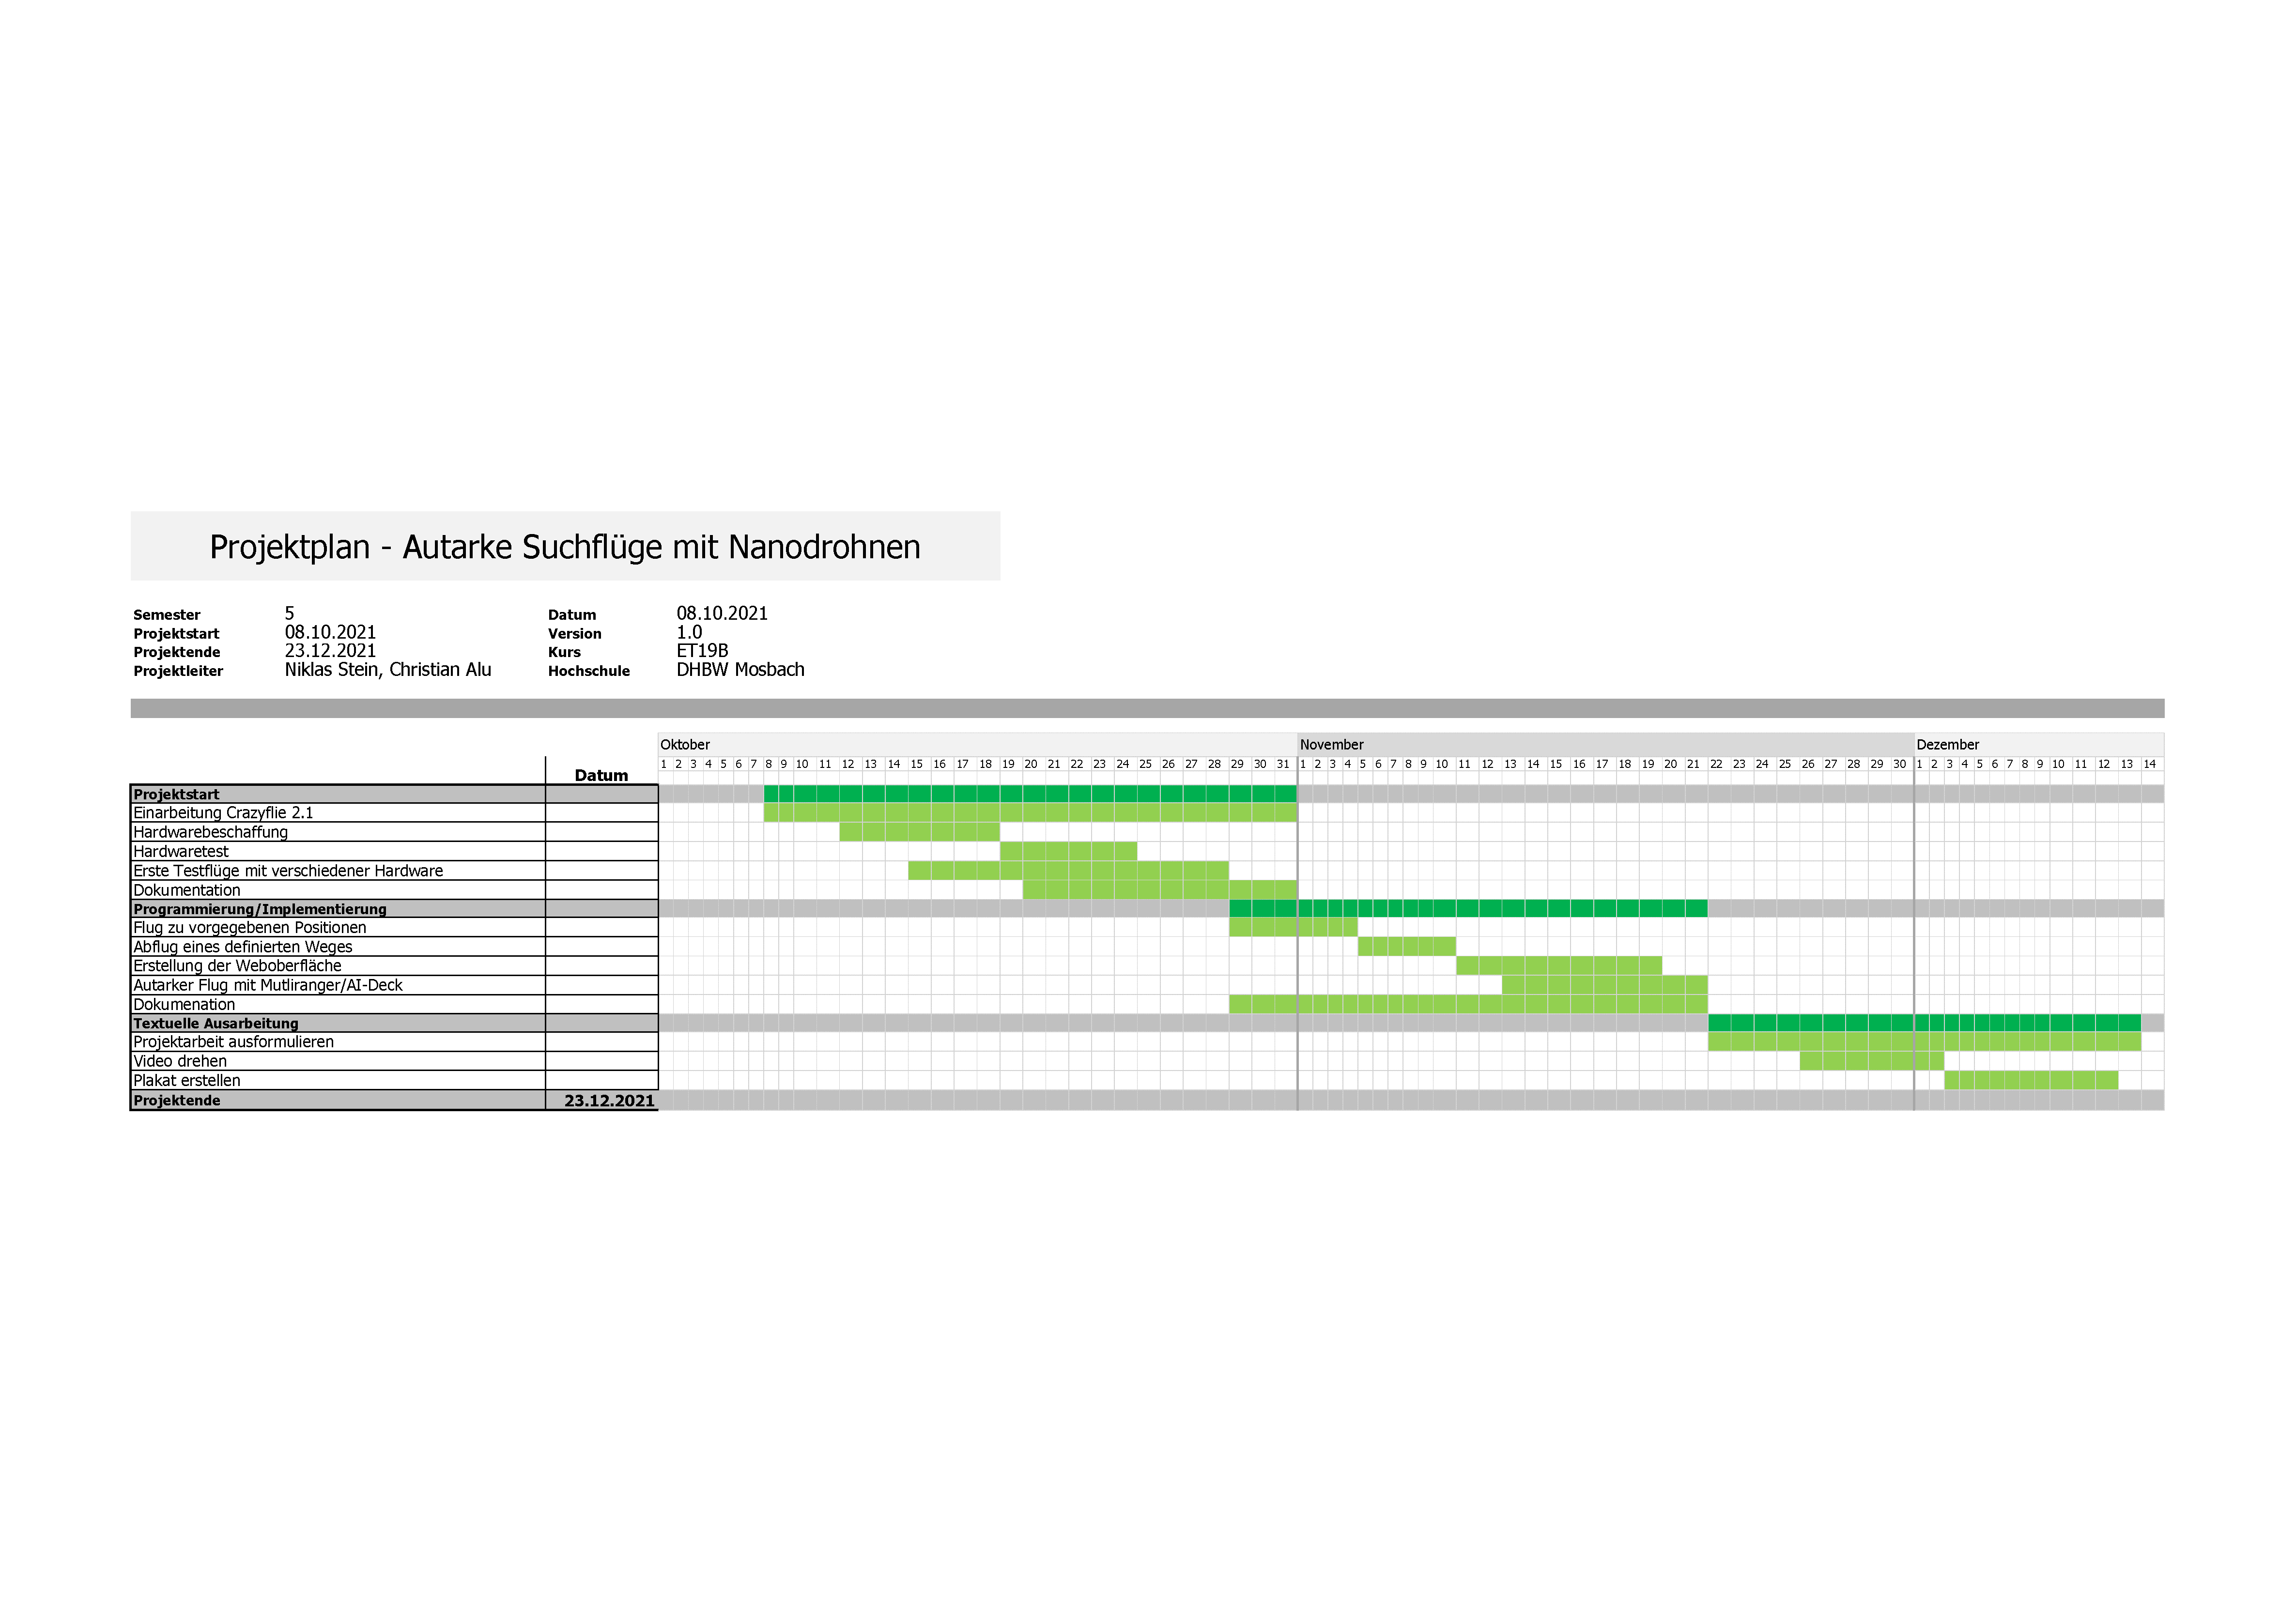
\includegraphics[angle=90, page=1,width=0.85\textwidth]{anhang/Projektplan.pdf}
	\caption{Zeitplan der Projektarbeit im 5. Semester  \protect \\ Quelle: Eigene Darstellung}
	\label{lab:Projektplan}
\end{figure}



\chapter{Datenblätter}
\newpage
	\section{Crazyflie 2.1}
	\begin{figure}[H]
	\centering
	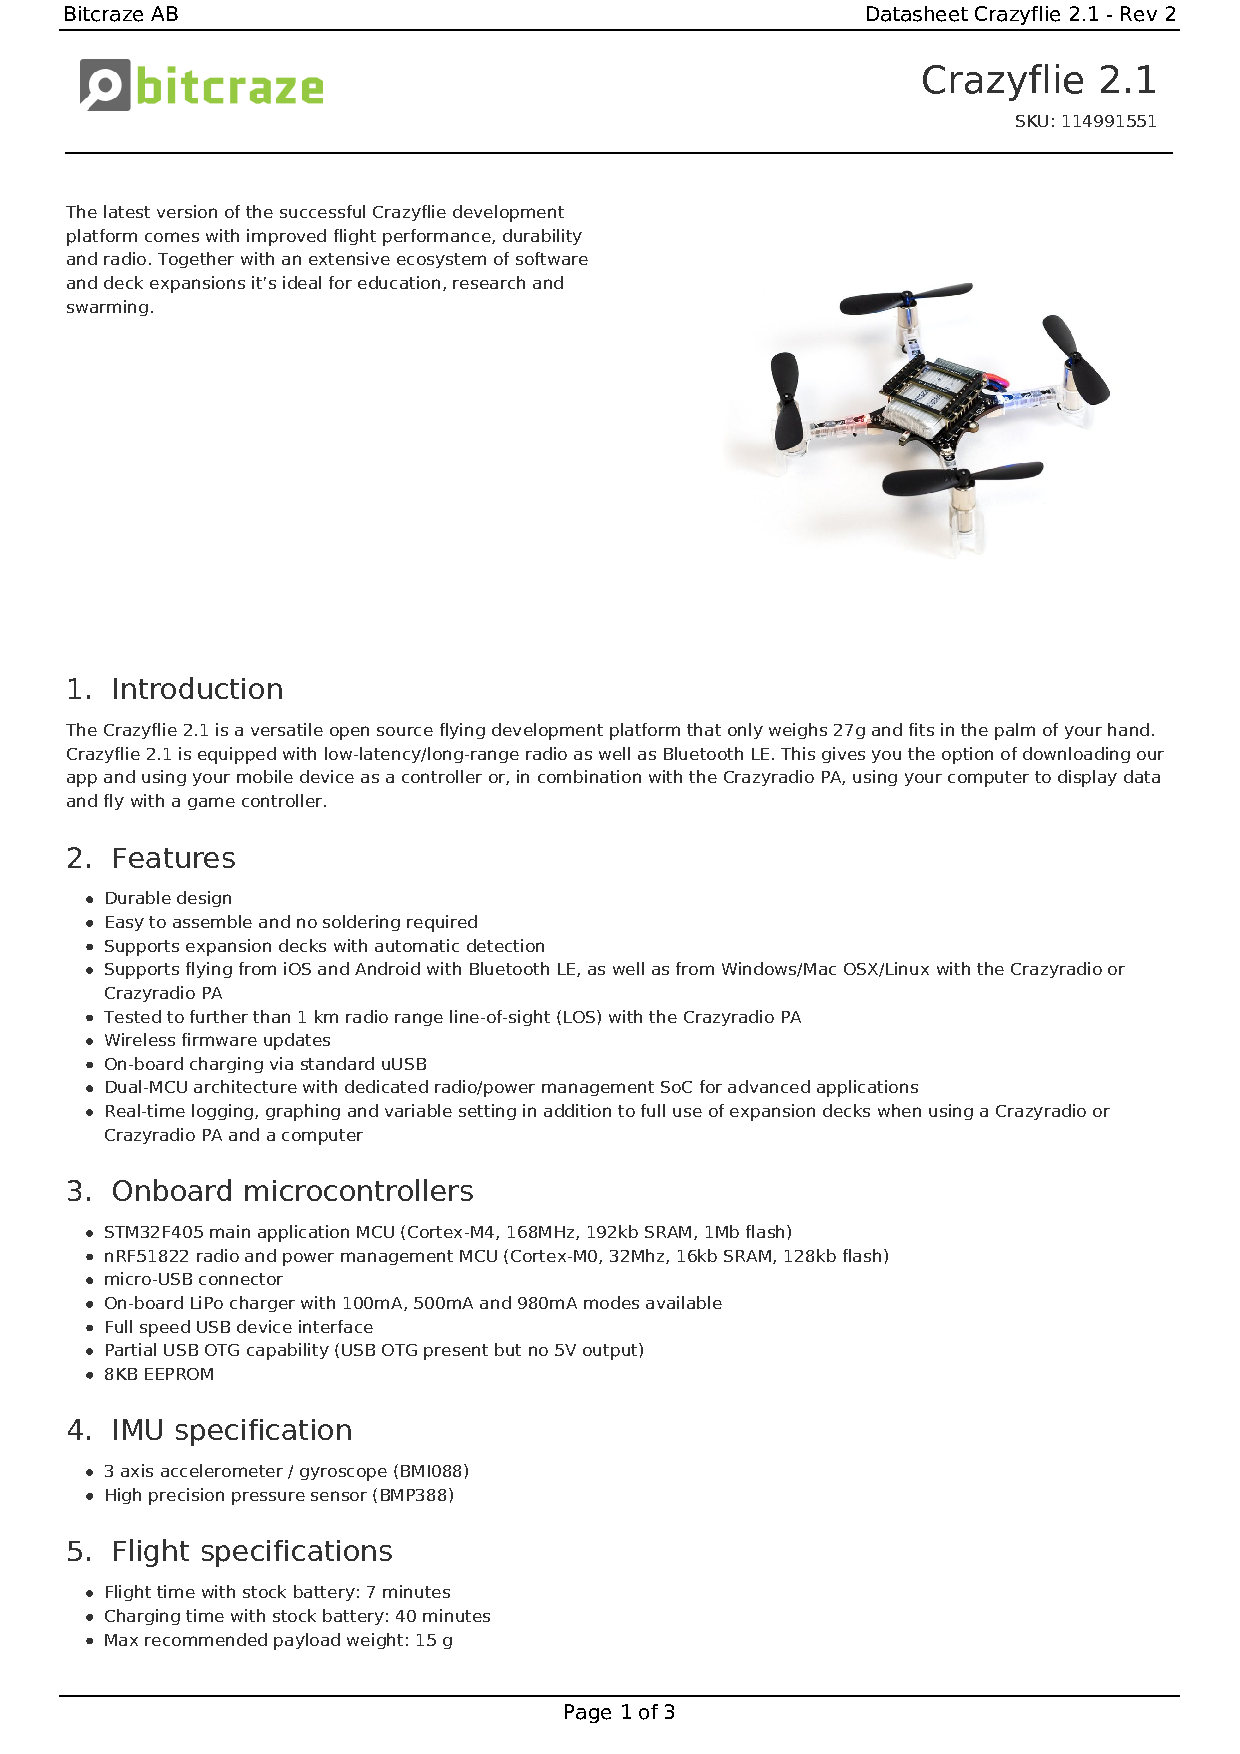
\includegraphics[page=1,width=.8\textwidth]{anhang/crazyfliedatasheet.pdf}
\end{figure}

	\begin{figure}[H]
	\centering
	\includegraphics[page=2,width=.8\textwidth]{anhang/crazyfliedatasheet.pdf}
\end{figure}

	\begin{figure}[H]
		\centering
		\includegraphics[page=3,width=.8\textwidth]{anhang/crazyfliedatasheet.pdf}
		\caption{Datenblatt Crazyflie 2.1 \protect \\ Quelle: \cite{.} }
		\label{lab:crazyfliedatasheet.pdf}
	\end{figure}


	
\end{document}